%%%%%%%%%%%%%%%%%%%%%%%
%%  Capítulo 4: Aplicación a estructras microstrip  %%
%%%%%%%%%%%%%%%%%%%%%%%

%%%%

\section{Introducción}

El análisis del capítulo 3 permite comprender de forma intuitiva el comportamiento de las estructuras EBG uniplanares dispuestas sobre un plano de tierra cubierto por sustrato dieléctrico. Sin embargo, el análisis sólo se propuso para energía conducida, debida al comportamiento de corrientes sobre el metamaterial que dan lugar a una modificación en la estructura y capacidad de propagación de ondas. Este análisis, si bien importante para la comprensión de los efectos ligados a las estructuras periódicas, no se centra en el análisis del comportamiento de las mismas en cercanías de radiadores electromagnéticos.

En este capítulo se iniciará, aunque no se concluirá completamente, el estudio sobre el efecto de estas estructuras sobre las propiedades de radiación y de campo cercano de antenas ubicadas sobre el sustrato. El análisis comenzará con la revisión del comportamiento cuando las antenas en cuestión son monopolos eléctricos referenciados al plano conductor inferior, y una vez destacados los efectos más importantes que se dan para este tipo de antenas, se procederá a mostrar los efectos para el caso en que los radiadores son antenas microstrip, en que aparecen fenómenos más complejos.

El motivo por el que se comienza el análisis para monopolos eléctricos verticales gira en torno a la capacidad que estos poseen para generar, sobre la capa dieléctrica, ondas de superficie TM en forma isotrópica, sin efectos de borde ni asimetrías que dificulten el análisis.

\section{Monopolos}

Las antenas monopolo consisten en un conductor dispuesto verticalmente sobre un plano de tierra u otra superficie conductora, alimentado o conectado a un receptor en su base a través de una línea de transmisión cuyos terminales están conectados al plano de tierra y al conductor vertical respectivamente, como se muestra en la figura \ref{fig:monopolos} b). A diferencia del dipolo, que consiste en dos conductores idénticos dispuestos de forma tal que comparten su eje principal, el monopolo suele ser más corto, posee un diagrama de radiación más elevado (como se observa en la figura \ref{fig:monopolos} a)), una resistencia de radiación menor, una mayor directividad, y da lugar a ondas de superficie considerables sobre el plano conductor.


\begin{figure}[H]
	\centering 
	\subfigure[Diagrama de radiación de un monopolo de longitud $2\lambda/3$.]{
		\label{fig:diag-rad-monopolo}
		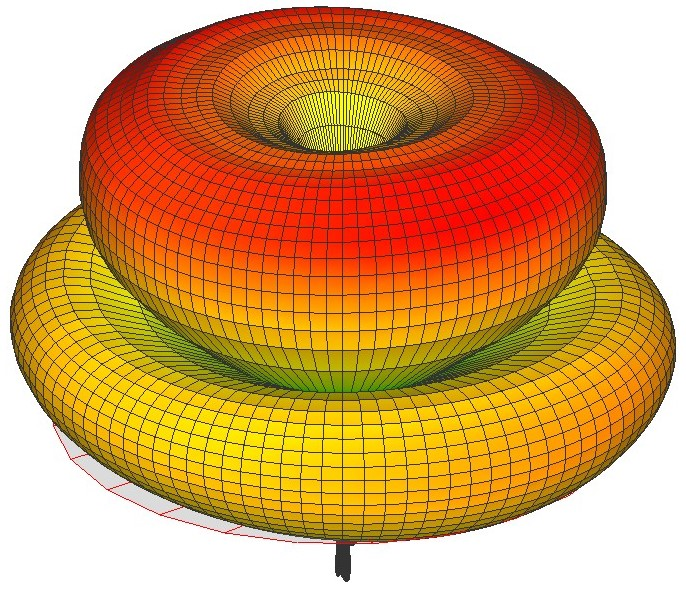
\includegraphics[width=0.30\textwidth]{Aplicacion/diagrad-monopolo-wikipedia.jpg}}
	\hspace{30pt}
	\subfigure[Diagrama de una antena monopolo.]{
		\label{fig:monopolo}
		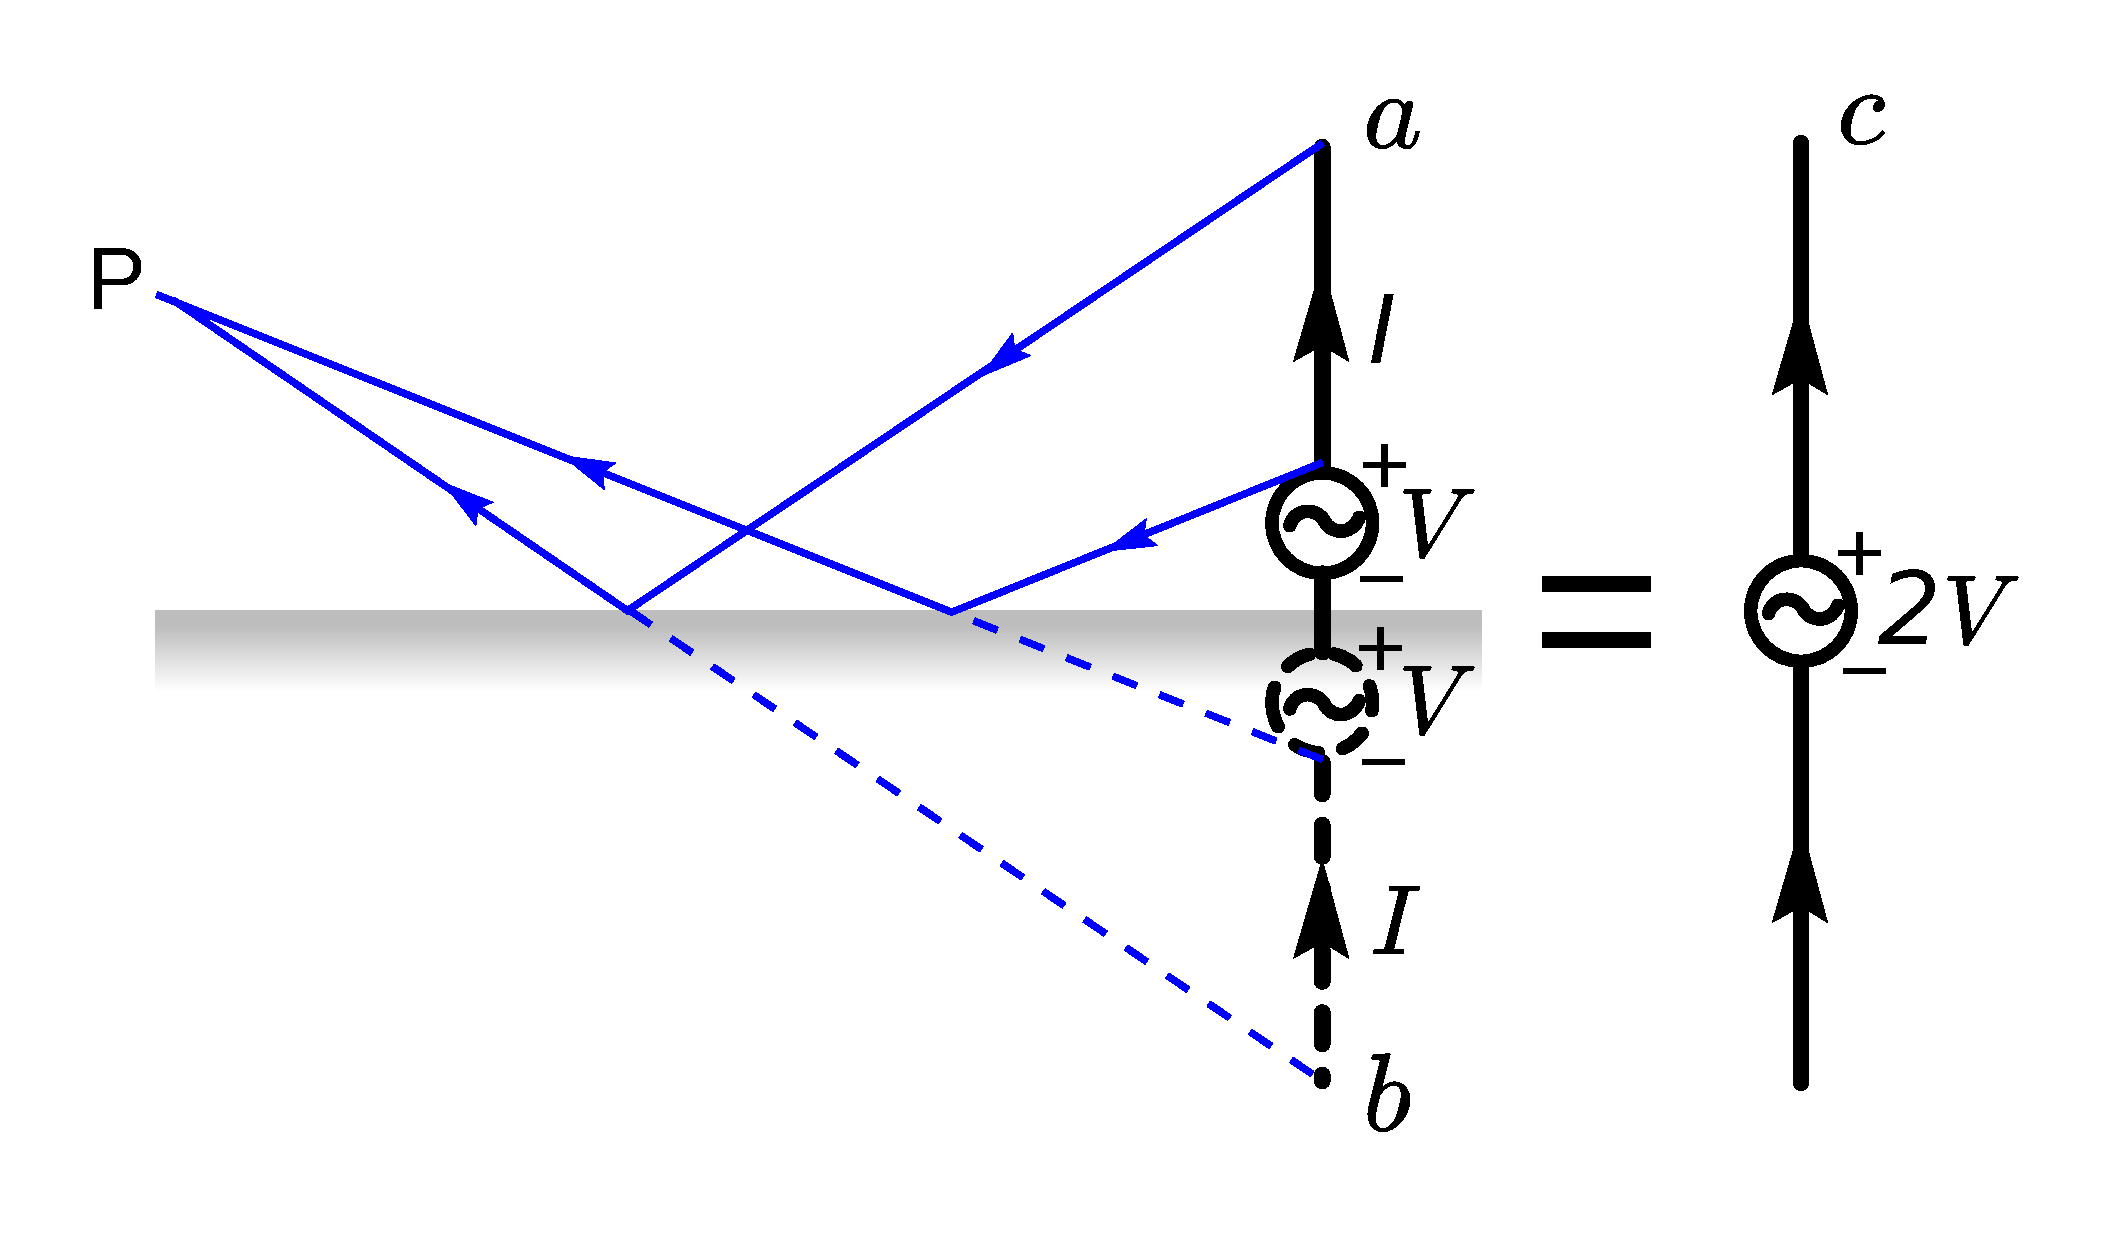
\includegraphics[width=0.50\textwidth]{Aplicacion/Monopole_and_image_antenna.pdf}}
	\caption{Imágenes extraídas de \textit{Wikipedia}.}
	\label{fig:monopolos}
\end{figure}


El análisis de un monopolo suele derivar de la aplicación de teoría de imágenes sobre un dipolo dispuesto a cierta distancia del plano de tierra. Este método de análisis genera fuentes virtuales de radiación bajo el plano conductor que, combinadas con las fuentes reales (el conductor vertical del monopolo), dan lugar a un sistema equivalente para la zona del espacio que se ubica por encima del plano de tierra, dado que describe las reflexiones sobre el mismo. Las fuentes virtuales tienen, sobre un plano conductor, el comportamiento mostrado en la figura \ref{fig:fuentes-virtuales}.


\begin{figure}[h]
	\centering
	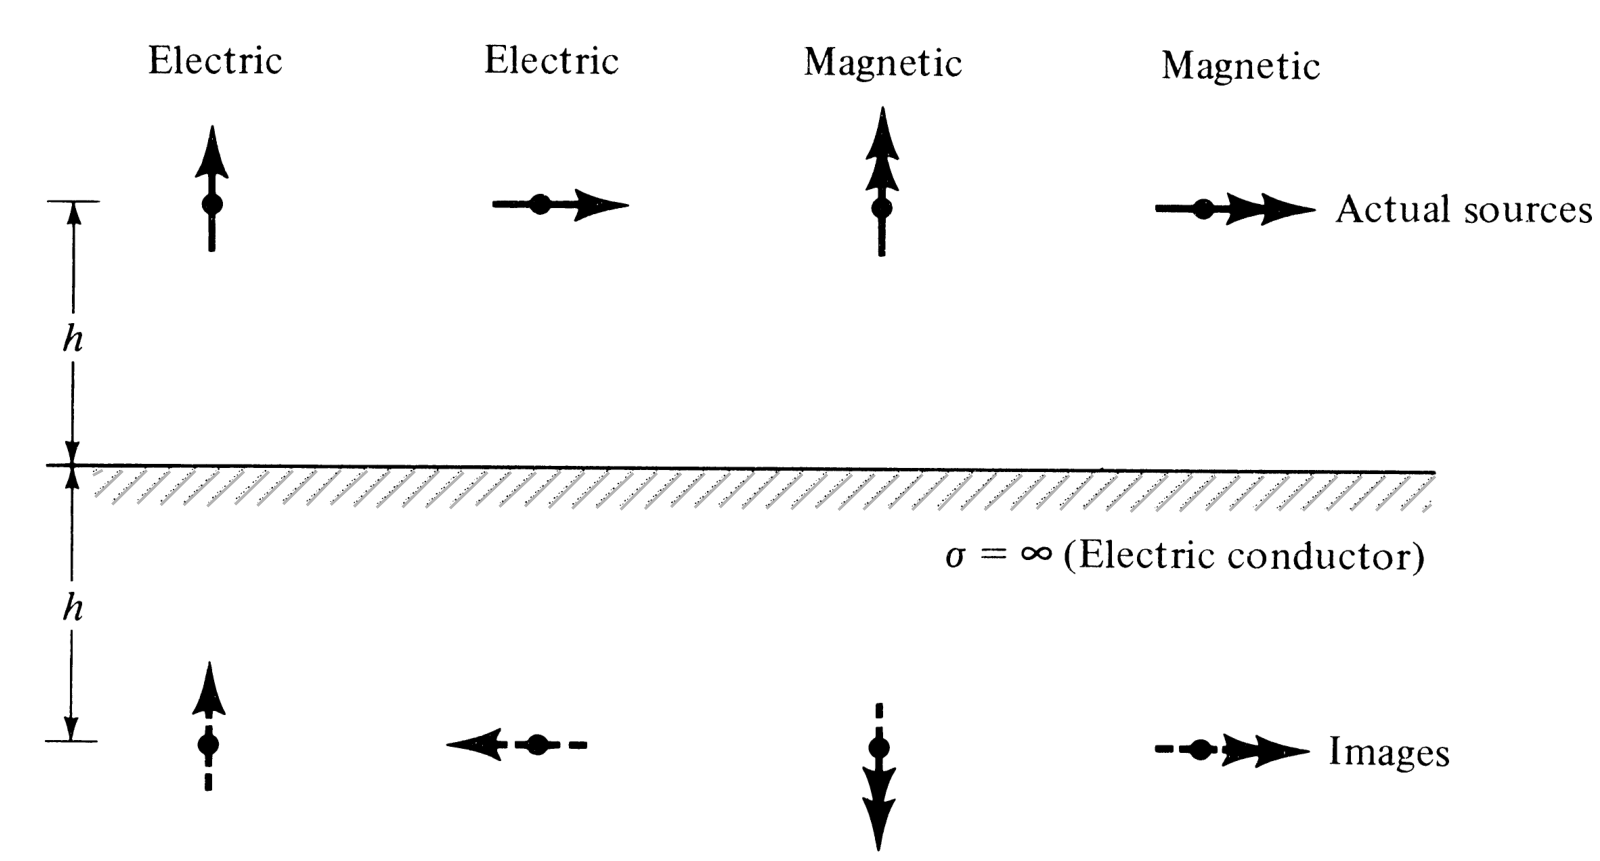
\includegraphics[width=1\textwidth]{Aplicacion/balanis-metodo-imagenes.PNG}
	\caption{Fuentes virtuales generadas por cercanía con un conductor eléctrico \cite{Balanis:Theory}.}
	\label{fig:fuentes-virtuales}
\end{figure}

\subsection{Comportamiento de un arreglo de dos monopolos}

Para las pruebas sobre acoplamiento mutuo que se realizaron, se consideró un monopolo de $\lambda/4$, que para la frecuencia de interés es de aproximadamente $3.125\;cm$. Se ubicaron dos monopolos a una distancia arbitraria de $6.25\; cm$ sobre un plano conductor finito cubierto por un sustrato de FR-4, a fin de conocer el acoplamiento entre ambas antenas cuando no existe una estructura de \textit{bandgap} electromagnético entre ellas. La geometria creada se puede observar en la figura \ref{fig:dos-monopolos}. Se debe considerar que, como se explicó en la sección \ref{subsec_acoplamiento}, el acoplamiento entre antenas se debe a múltiples factores, y el uso de estructuras EBG en el sustrato será responsable de únicamente uno de ellos: las ondas de superficie.

\begin{figure}[h]
	\centering
	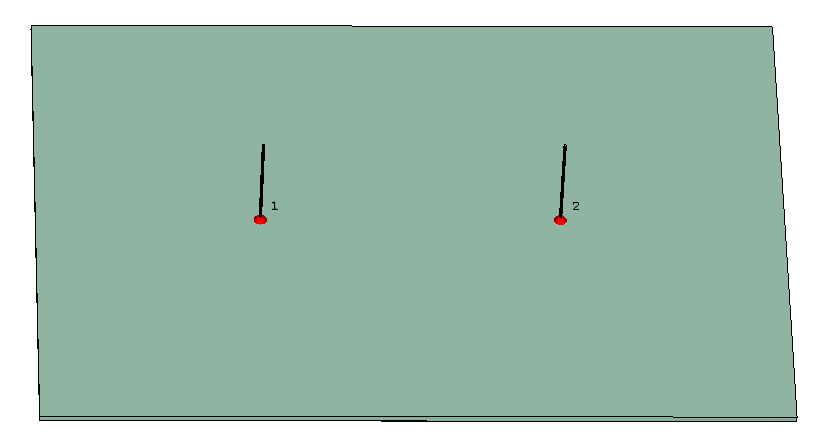
\includegraphics[width=0.7\textwidth]{Aplicacion/dos-monopolos.png}
	\caption{Estructura de dos monopolos sobre un plano de tierra simulada.}
	\label{fig:dos-monopolos}
\end{figure}

Por el motivo antes comentado, si las antenas se ubicaran demasiado cerca, la intensidad relativa de los efectos debidos al acoplamiento por campo cercano serían mucho mayores a los del acoplamiento por ondas de superficie, de forma que en muchos casos, en lugar de mejorar el comportamiento, el uso de EBGs lo empeorará, sumando más efectos negativos que positivos. Estas estructuras resultarán útiles sólo en aquellos casos en que la distancia entre los radiadores sea lo suficientemente grande como para poder considerar efectos de acoplamiento relacionados a la propagación de ondas de superficie.

Se varió la distancia para conocer la variación del coeficiente de acoplamiento con la misma. Los resultados se muestran en la figura \ref{fig:dipolos-distancia-resultados} donde, como resultaba esperable, el mismo disminuye con la distancia, y la frecuencia de resonancia del mismo aumenta ligeramente a medida que los dipolos se alejan, modificando de forma casi insignificante el nivel de adaptación.

\begin{figure}[h]
	\centering 
	\subfigure[Parámetro $S_{11}$.]{
		\label{fig:dipolos-s11-variasDistancias-sinEBG}
		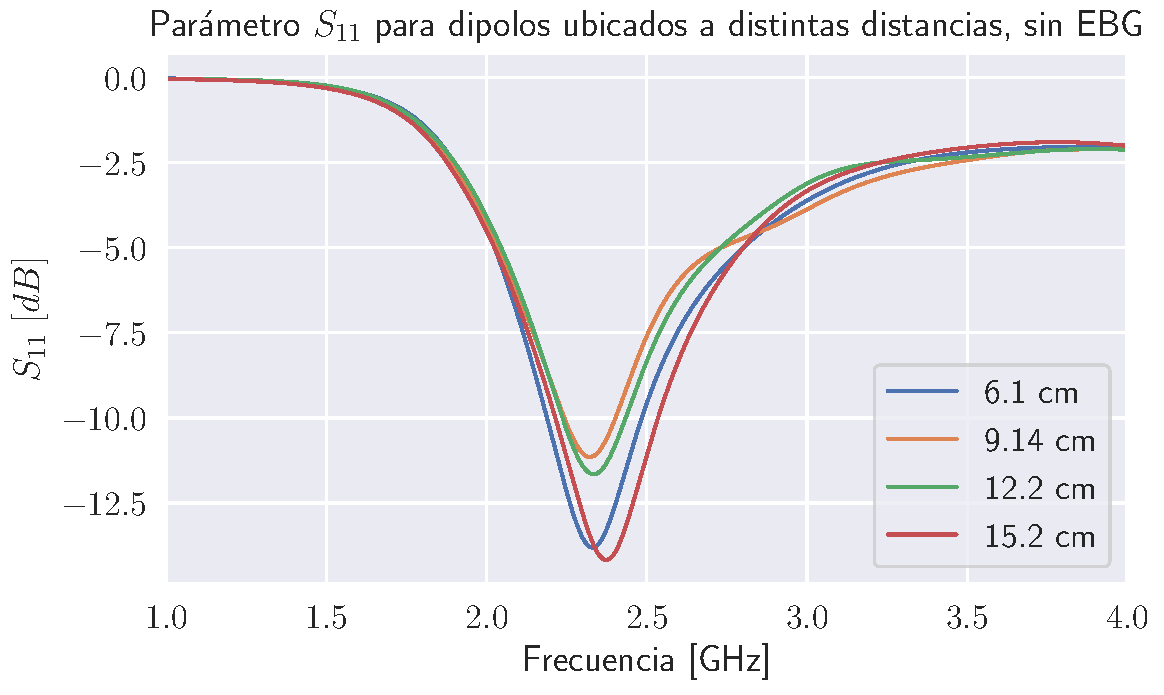
\includegraphics[width=0.45\textwidth]{Aplicacion/dipolos-s11-variasDistancias-sinEBG.pdf}}
	\hspace{0pt}
	\subfigure[Parámetro $S_{12}$.]{
		\label{fig:dipolos-s12-variasDistancias-sinEBG}
		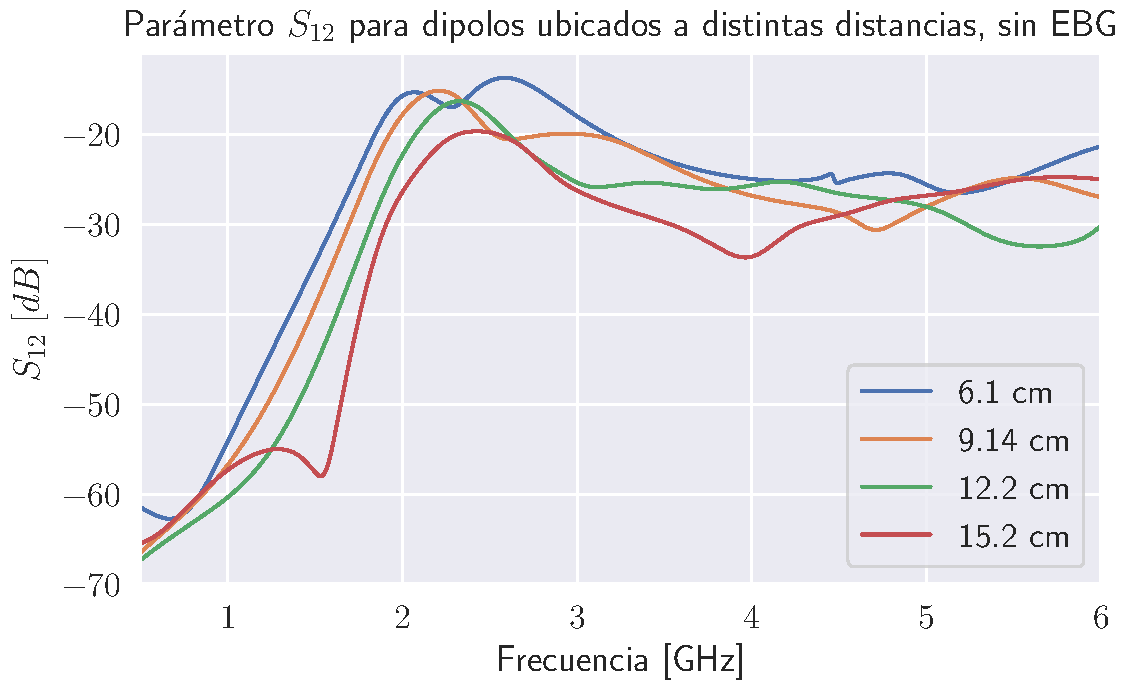
\includegraphics[width=0.45\textwidth]{Aplicacion/dipolos-s12-variasDistancias-sinEBG.pdf}}
	\caption{Comportamiento de los parámetros S para dos dipolos ubicados a distintas distancias.}
	\label{fig:dipolos-distancia-resultados}	
\end{figure}  

En vistas de comprender la incidencia del acoplamiento por ondas de superficie sobre el acoplamiento total entre ambas antenas, se eliminó el plano de tierra que se ubica entre ambos dipolos. Esto tiene consecuencias muy notorias sobre el diagrama de radiación, pues deja de existir el plano conductor y, por tanto, la fuente de campo virtual que se consideraba en la figura \ref{fig:monopolos} b) ya no existe. El comportamiento del parámetro $S_{21}$ para el caso en que no hay un plano de tierra completo que vincule a ambas antenas se pueden observar en la figura \ref{fig:monopolos-sin-plano-de-tierra-resultados}, que surge de la simulación de la figura \ref{fig:monopolos-sin-plano-de-tierra-geometria}. 


\begin{figure}[h]
	\centering
	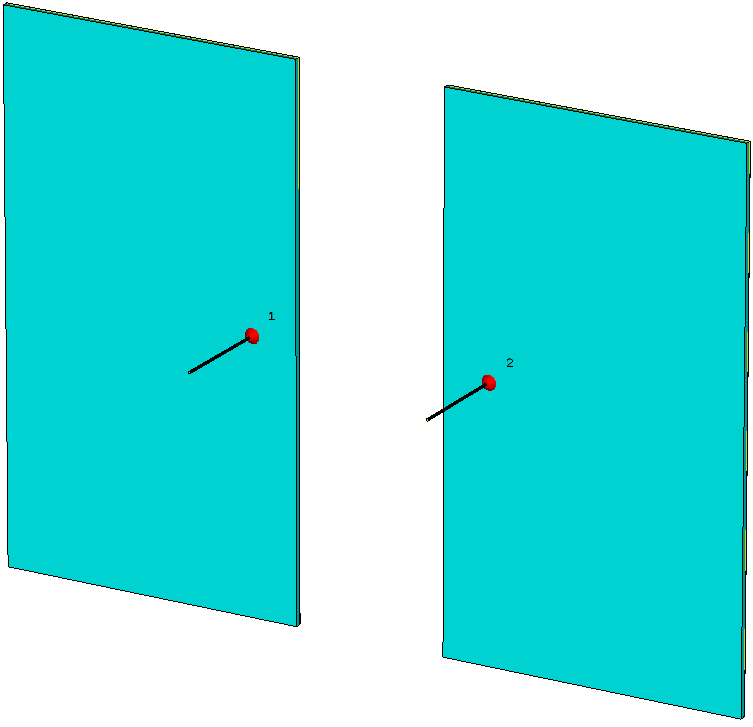
\includegraphics[width=0.5\textwidth]{Aplicacion/dos-monopolos-sin-GND.png}
	\caption{Estructura de dos monopolos ubicados sobre dos planos conductores separados para evitar acoplamiento por ondas de superficie.}
	\label{fig:monopolos-sin-plano-de-tierra-geometria}
\end{figure}

\begin{figure}[h]
	\centering 
	\subfigure[Parámetro $S_{11}$.]{
		\label{fig:dipolos-s11-variasDistancias-sinGND}
		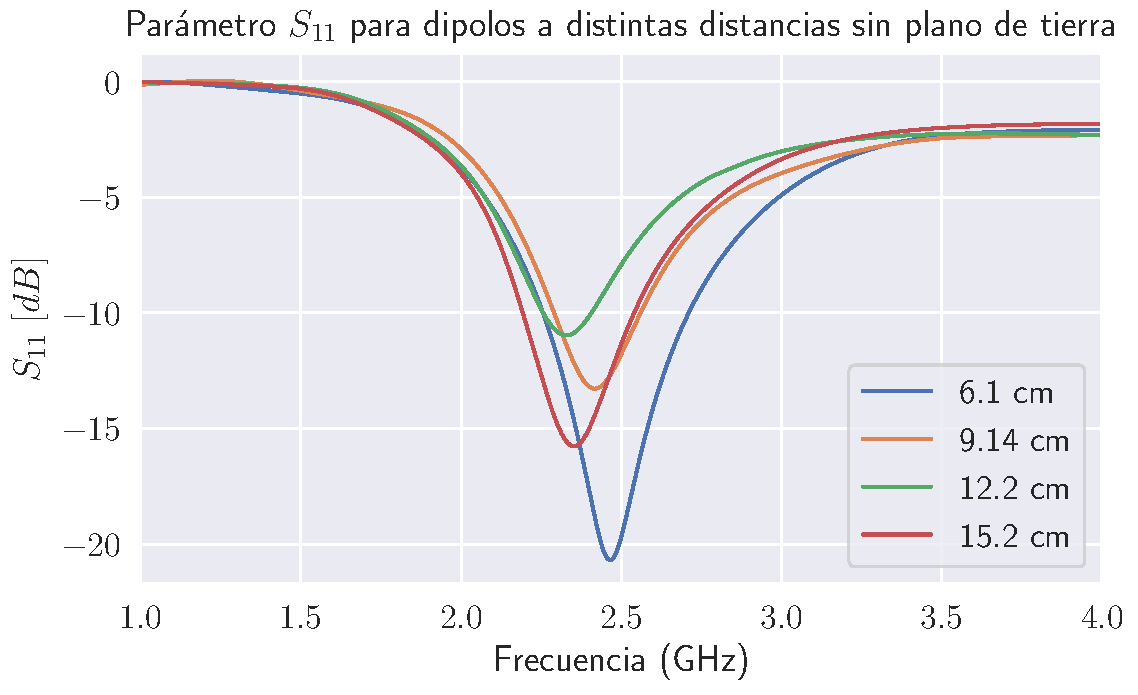
\includegraphics[width=0.45\textwidth]{Aplicacion/dipolos-s11-variasDistancias-sinGND.pdf}}
	\hspace{0pt}
	\subfigure[Parámetro $S_{12}$.]{
		\label{fig:dipolos-s12-variasDistancias-sinGND}
		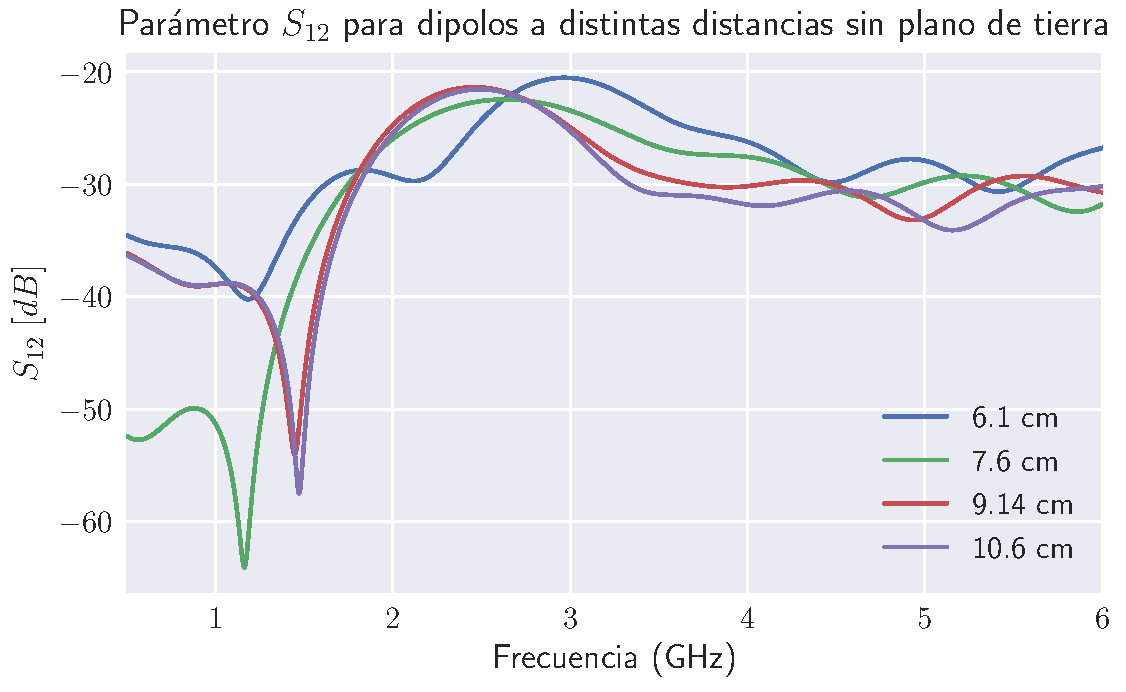
\includegraphics[width=0.45\textwidth]{Aplicacion/dipolos-s12-variasDistancias-sinGND.pdf}}
	\caption{Comportamiento de los parámetros S para dos dipolos ubicados a distintas distancias, con un plano de tierra dividido en dos para evitar acoplamiento por ondas de superficie.}
	\label{fig:monopolos-sin-plano-de-tierra-resultados}	
\end{figure}  

Se puede observar que los valores de distancia para los que los monopolos quedan cerca del borde de su respectivo plano conductor y del radiador opuesto, la adaptación del sistema mejora considerablemente. A medida que las antenas se alejan, el parámetro $S_{11}$ recupera los valores que poseía cuando la estructura tenía un único de plano de tierra. Una comparación para dos distancias elegidas arbitrariamente se puede observar en la figura \ref{fig:comparacion-monopolos-s-sinGND} a). De la misma manera, el comportamiento en función de la frecuencia de las geometrías en que la distancia entre los monopolos, y entre cada uno de los radiadores y el borde del plano conductor, disminuye, el acoplamiento aumenta para las bajas frecuencias, y surgen efectos indeseados. Una comparación, también para dos distancias elegidas arbitrariamente, se observa en la figura \ref{fig:comparacion-monopolos-s-sinGND} b), donde se puede observar una disminución en el parámetro $S_{12}$ de unos $8\ dB$ para las frecuencias de interés, incluso cuando las antenas están lejos del borde que las enfrenta (curva naranja). Esto permite deducir, entonces, que el efecto de acoplamiento por ondas de superficie no es despreciable, aunque no representa, como se esperaba, la causa única del mismo.


\begin{figure}[h]
	\centering 
	\subfigure[Parámetro $S_{11}$.]{
		\label{fig:comparacion-dipolos-s11-variasDistancias-sinGND}
		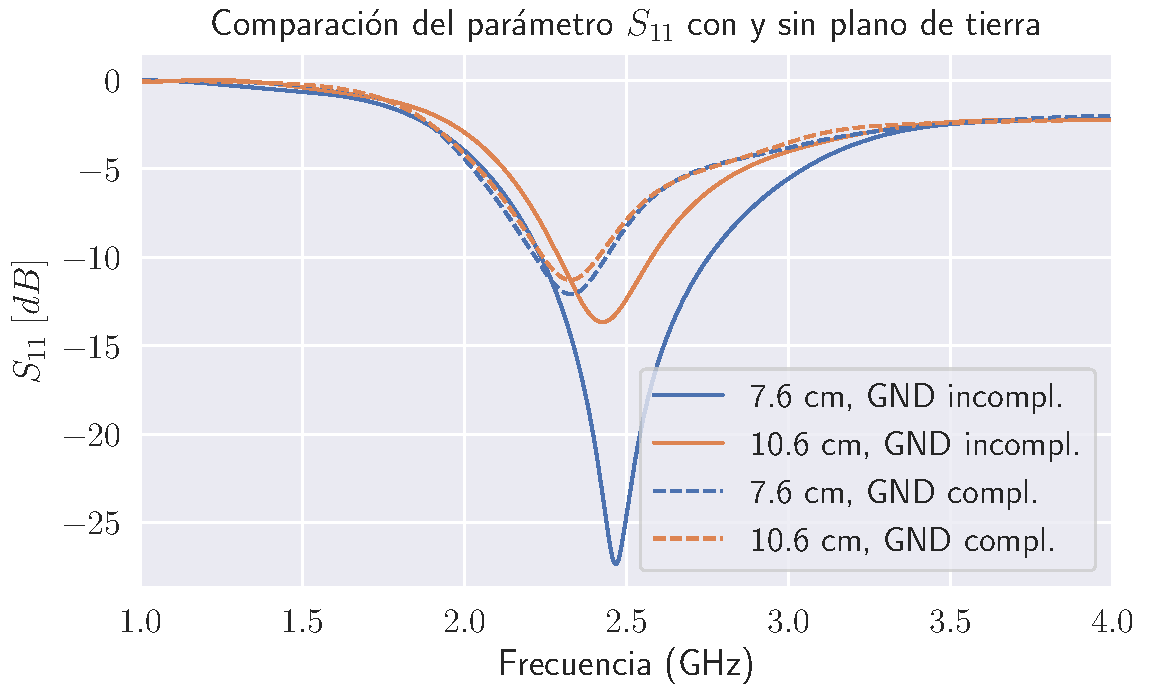
\includegraphics[width=0.45\textwidth]{Aplicacion/comparacion-dipolos-s11-variasDistancias-sinGND.pdf}}
	\hspace{0pt}
	\subfigure[Parámetro $S_{12}$.]{
		\label{fig:comparacion-dipolos-s12-variasDistancias-sinGND}
		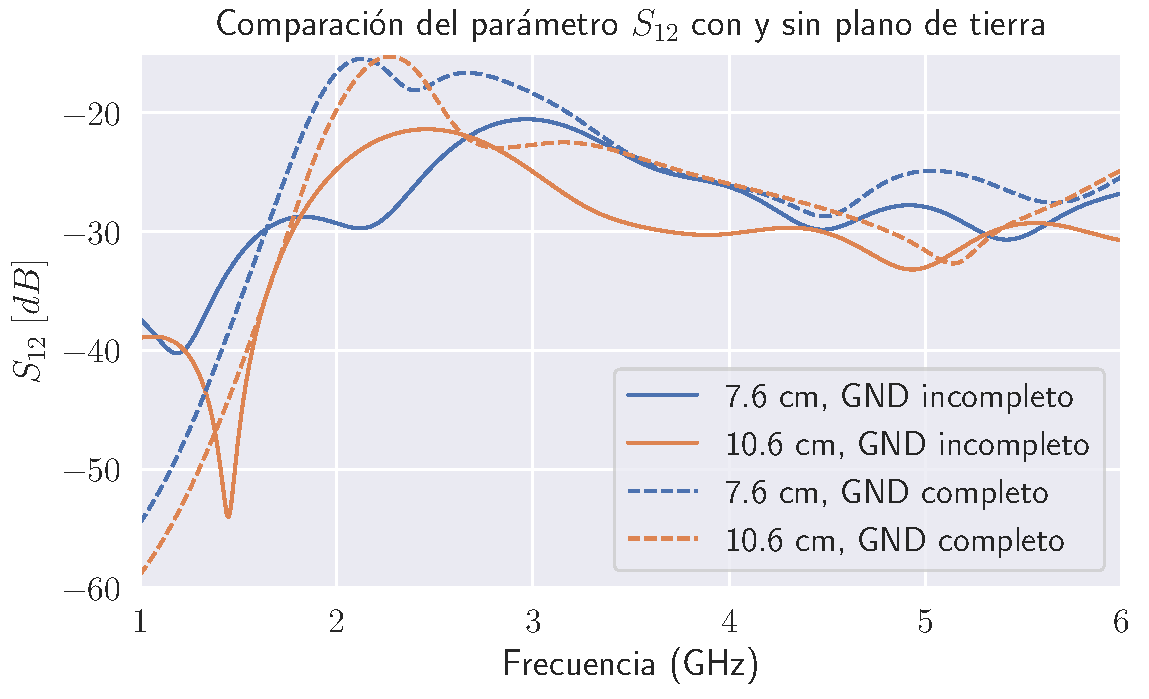
\includegraphics[width=0.45\textwidth]{Aplicacion/comparacion-dipolos-s12-variasDistancias-sinGND.pdf}}
	\caption{Comparación del comportameinto entre un par de monopolos que comparten plano conductor y un par de dipolos que no, para dos distancias entre antenas elegidas arbitrariamente.}
	\label{fig:comparacion-monopolos-s-sinGND}
\end{figure} 

	
\section{Introducción a antenas \textit{microstrip}}

Como se describió en la sección \ref{subsec_antenas_microstrip}, las antenas \textit{microstrip} son utilizadas en un amplio rango de aplicaciones comerciales y militares, especialmente debido a que son livianas, de bajo perfil, suponen reducidos costos y resultan de fácil fabricación. Además, permiten diseños integrados con componentes activos, circuitos de microondas y elementos radiantes \cite{Yang:EBGAntennas}.

El tamaño de las antenas está íntimamente ligado a la longitud de onda de trabajo, que se relaciona a la frecuencia y permitividad eléctrica del sustrato utilizado, como queda explícito en la ecuación \ref{eq:frecRes-modosSup-microstripAntenna}. Al mismo tiempo, dado que en general son antenas resonantes, presentan un alto Q, lo que afecta a su ancho de banda.

En muchos casos es necesario disminuir el tamaño de los elementos \textit{microstrip}, lo que se puede lograr mediante cortocircuitos y líneas \textit{microstrip} de formas complejas. Otro método, más sencillo, consiste en aumentar el valor de la permitividad eléctrica del sustrato. Sin embargo, como ya se explicó antes, y como se puede observar en la figura \ref{fig:zstm-permit-diel}, el aumento de este parámetro aumenta el valor de la impedancia inductiva de la superficie, permitiendo el desarrollo de ondas de superficie.

Por otro lado, el uso de dieléctricos de constante alta genera un ancho de banda aún menor (un mayor Q) y aún más baja eficiencia de radiación. Estos efectos suelen mitigarse con el aumento del ancho del sustrato, que, en contrapartida, genera condiciones propicias para la propagación de ondas de superficie en modo TM, debido a que, como se indica en la ecuación \ref{eq:campo-magnetico-interior-diel-TM} y se esquematiza en la figura \ref{fig:soluciones-TM-tan-implicita-zoom}, se permiten una mayor cantidad de modos de propagación en el eje $x$ (vertical). Por otro lado, un análisis de la impedancia de superficie indica que el comportamiento inductivo aumenta con el ancho del sustrato (ecuación \ref{eq:impedancia-superficie-tm-teorica} y figura \ref{fig:Zstm-parametros}), lo que también es signo de una configuración que soporta ondas de superficie con facilidad.

Las ondas de superficie, además, extraen potencia que no se convierte en radiación y, facilitan el acoplamiento entre elementos. Además, cuando inciden sobre discontinuidades, generan lóbulos secundarios que degradan el patrón de radiación y las características de polarización \cite{Balanis:Theory}.

Entre las distintas técnicas que han surgido para la disminución de la presencia de ondas de superficie en el sustrato que soporta a las antenas \textit{microstrip}, entre las que destacan las relativas a disminuir la altura del sustrato en los bordes de la antena (figura \ref{fig:escalon-sustrato}), en los últimos años ha cobrado especial interés el uso de sustratos con banda prohibida electromagnética, debido a que no requieren un cambio en la tecnología de fabricación. Los mismos pueden aplicarse justo debajo de la antena (generando estructuras planares que reemplazan al plano de tierra, conocidas como DGS, que ofrecen como contrapartida un diagrama de radiación con mayores lóbulos laterales), o alrededor de la misma (\cite{Marcela:Tesis}, figura \ref{fig:sustrato-antena-ebg}). Ambas soluciones, debido a la naturaleza resonante de la antena, que genera que las frecuencias en juego estén distribuidas en un ancho de banda acotado, tienen como consecuencia una disminución del acoplamiento mutuo con elementos circuitales cercanos a la antena (en particular, otras antenas que podrían estar formando parte de un arreglo de radiadores). Esto es así porque, si las estructuras que rodean al elemento radiante tienen una banda prohibida para las frecuencias de trabajo, las mismas no podrán propagarse por el sustrato.


\begin{figure}[H]
	\centering 
	\subfigure[Antena rodeada por una estructura EBG.]{
		\label{fig:sustrato-antena-ebg}
		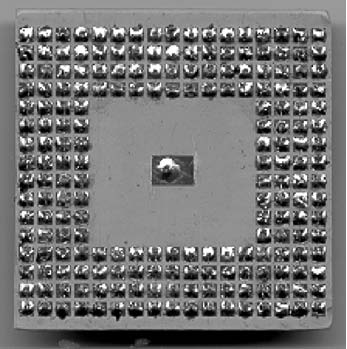
\includegraphics[width=0.40\textwidth]{Aplicacion/foto-ebg-alrededor-antena.pdf}}
	\hspace{30pt}
	\subfigure[Antena rodeada por un escalón de sustrato,]{
		\label{fig:escalon-sustrato}
		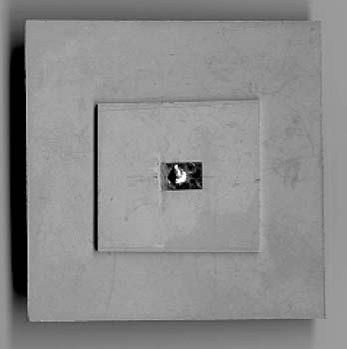
\includegraphics[width=0.40\textwidth]{Aplicacion/foto-escalon-alrededor-antena.pdf}}
	\caption{Fotos de diseños de antenas parches con limitadores a la propagación de onda de superficie \cite{Yang:EBGAntennas}.}
	\label{fig:limitadores-ondas-superficie-yang}
\end{figure}

Las primeras estructuras EBG utilizadas con estos fines consistían en arreglos de agujeros cilíndricos en el sustrato que, debido a la periodicidad que presentaban para las ondas de superficie, daban lugar a un comportamiento de filtro, presentando una banda prohibida. La dificultad para la fabricación de este tipo de sustratos dio lugar a la búsqueda de estructuras de banda prohibida de mayor facilidad de uso. En 1999, Sievenpiper presentó, en sus tesis doctoral \cite{Sievenpiper:Thesis}, una estructura que denominó HIS (\textit{High Impedance Surface}, superficie de alta impedancia), que además de cumplir con las características de un conductor magnético para un rango de frecuencias \cite{Sievenpiper:HIESForbiddenBand} y de ser de fácil fabricación con tecnología \textit{microstrip}, poseía también una banda prohibida electromagnética para las ondas de superficie \cite{Marcela:Tesis}. Esta estructura, consistente en parches metálicos dispuestos sobre un sustrato, y unidos al plano de tierra, ubicado en la cara opuesta del mismo, a través de vías metálicas, redujo ampliamente los costos y la dificultad de fabricación. Pocos años más tarde, debido a que en algunos casos el uso de vías retrasa la fabricación de circuitos \textit{microstrip}, surgieron estructuras de banda prohibida uniplanares, con características similares, aunque con anchos de banda prohibida más reducidos.

Para el presente trabajo, estas estructuras se ubicarán entre dos antenas microstrip, alineadas según distintos criterios, a fin de comparar el diagrama de radiación y el acoplamiento mutuo con el que se logra con el mismo arreglo radiante, pero sin el uso de EBG entre ellas.

% Coccioli, Yang, Itoh, intro historica.
%%%%
\section{Diseño de una antena \textit{microstrip}}
\label{sec_disenio_microstrip}
%%%%
Para el diseño de una antena microstrip, se deben utilizar los modelos teoricos analizados en la sección \ref{sec:modelo_analitico}. Se debe calcular, en primer lugar, un valor tentativo del ancho W de la antena (con W según la figura \ref{fig:antema-microstrip-inset} a)), teniendo en cuenta que un mayor ancho W da lugar a una menor resistencia de entrada $R_{in}$. Una fórmula empírica está dada por \cite{Barthia:Handbook}, y para una frecuencia de resonancia de unos 2.42 GHz y sustrato FR-4 de 1.6 mm de espesor, resulta:

\begin{align}
	W = \frac{c_0}{2 f_r} \sqrt{\frac{2}{\epsilon_r+1}} = 37.35\; mm
\end{align}

Obtenido el ancho aproximado, se puede calcular la permitividad eléctrica eficaz, $\epsilon_{eff}$, de la ecuación \ref{eq:cte-diel-efectiva-microstrip}, que resulta 4.17. Esto permite, conociendo la frecuencia de resonancia buscada, calcular la longitud efectiva de la línea de transmisión, como:

\begin{align}
	L_{eff} = \frac{c_0}{2 f_r \sqrt{\epsilon_{r_{eff}}}} = 30.32\; mm
\end{align}

Dado que $L_{eff} = L + 2 \Delta L$, a partir del cálculo de $\Delta L$, que cuantiza el efecto del \textit{fringing} sobre la frecuencia de resonancia, usando la expresión \ref{eq:deltaL-antena-microstrip}, que resulta en 0.74 mm, se puede saber el valor de L a utilizar ($L = L_{eff} - 2 \Delta L$), que es de 28.85 mm.

Además de la antena, debe diseñarse también la alimentación de la misma. De entre las múltiples formas de alimentación de una antena \textit{microstrip} \cite{Barthia:Handbook}, la seleccionada, en este trabajo, por su facilidad de fabricación, es la que consiste en una línea de la misma tecnología, que vincula a un conector en el borde de la placa con el parche, esquematizado antes en la figura \ref{fig:antema-microstrip-inset}. En particular, es importante que la impedancia característica de la línea \textit{microstrip} utilizada sea de $50\;\Omega$, para lo que debe seleccionarse con cuidado su ancho, en función de la altura del sustrato y la permitividad del dieléctrico. Según las expresiones que se pueden hallar en el Apéndice B de \cite{Barthia:Handbook}, el ancho necesario para obtener una impedancia de $50\;\Omega$ es de aproximadamente 3.1 mm.

Conocidos estos valores, resta determinar el \textit{inset} que debe aplicarse para obtener una impedancia de entrada de 50 $\Omega$, a fin de lograr adaptación entre la línea \textit{microstrip} de alimentación y el parche radiantec. Para esto, se debe utilizar la curva de la figura \ref{fig:antema-microstrip-inset} b), conociendo previamente el valor de la impedancia sobre el borde del parche rectangular. A partir de las expresiones de la parte real de la admitancia, o conductancia, obtenidas de \cite{Balanis:Theory} y mostradas en las ecuaciones \ref{eq:conductancia-microstrip-balanis} (donde $J_0$ es una función de Bessel del primer tipo de orden cero), la resistencia de entrada resulta $R_{in} = 1/[2(G_1 \pm G_{12})]$. A partir de este valor, la consulta a la gráfica permite deducir que el valor de \textit{inset} requerido es de aproximadamente 10.73 mm.

\begin{align}
	\label{eq:conductancia-microstrip-balanis}
	G_1 &= \frac{1}{\pi \eta_0} \int_0^\pi \left[ \frac{\sin \left( \frac{k_0 W}{2} \cos \theta \right) }{\cos \theta}\right]^2 \sin^3 \theta d\theta \\
	G_{12} &= \frac{1}{120 \pi^2} \int_0^{\pi} \left[ \frac{\sin \left( \frac{k_0 W}{2} \cos \theta \right) }{\cos \theta}\right]^2 J_o(k_0 L \sin \theta) \sin^3 \theta d\theta
\end{align}

El siguiente paso consiste en describir geométricamente la estructura calculada para el uso de un software de simulación que permita optimizar los parámetros, en vistas de que la frecuencia de resonancia sea 2.41 GHz, y que el parámetro $S_{11}$, correspondiente al puerto de alimentación, sea tan pequeño como sea posible. Es importante aclarar que el agregado de los parches de carga y de la estructura EBG modificará la frecuencia de resonancia, y que este análisis se realiza en miras de comprender los cambios que se producen sobre la antena original, y confirmar el aumento de ancho de banda mediante la técnica mencionada antes.

Los resultados de la variación de los tres parámetros de interés en el diseño de la antena, ya elegido el sustrato, se observan en la figura \ref{fig:simulaciones-microstrip-1parche}. Como se puede observar, en efecto de la variación del largo L es muy notorio, debido a que, como se explicó antes, modifica la frecuencia de resonancia: A mayor largo L, menor resulta la frecuencia de resonancia, debido a que la longitud de onda en resonancia es más corta. Se observa que para alrededor de 45 mm de largo, la frecuencia de resonancia ronda la buscada.

\begin{figure}[H]
	\centering 
	\subfigure[Variación del largo L.]{
		\label{fig:1parche-varlargo}
		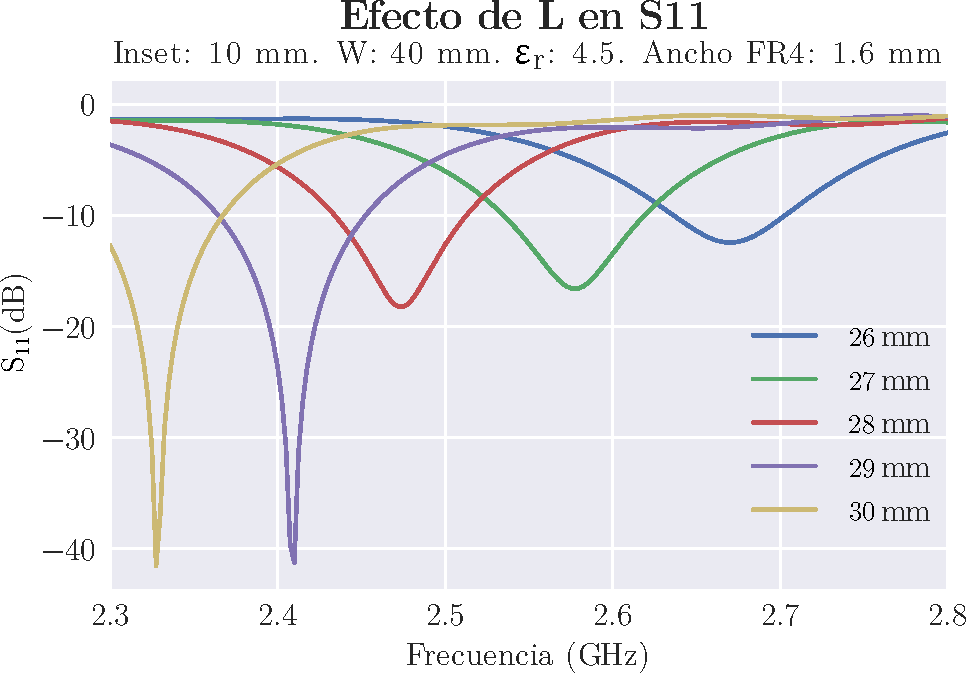
\includegraphics[width=0.48\textwidth]{Aplicacion/VariacionLargo-UnParche.pdf}}
	\subfigure[Variación del ancho W.]{
		\label{fig:1parche-varancho}
		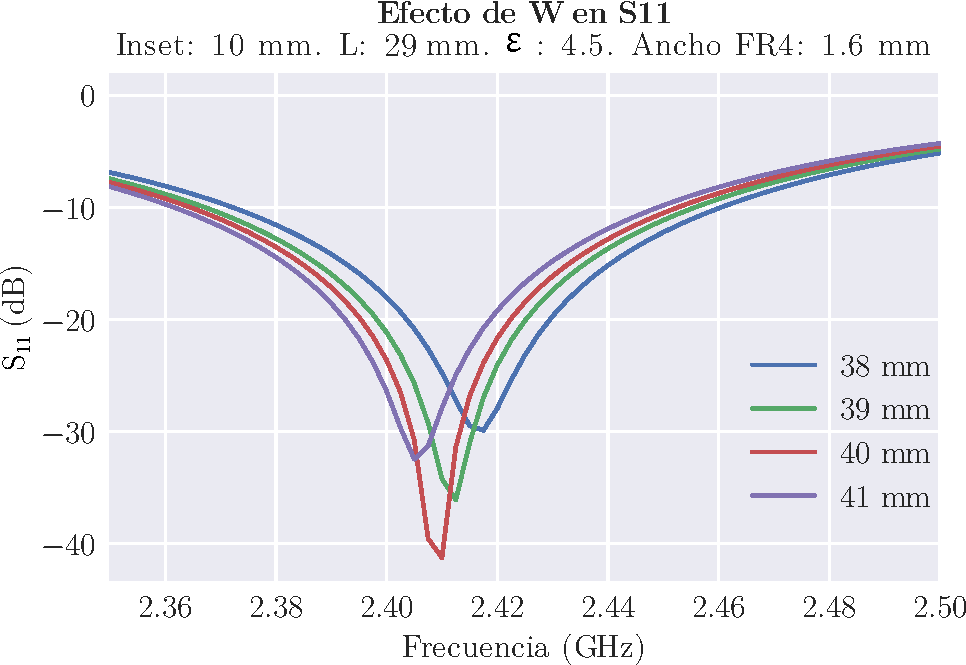
\includegraphics[width=0.48\textwidth]{Aplicacion/VariacionAncho-UnParche.pdf}}
	\subfigure[Variación de valor del \textit{inset}.]{
		\label{fig:1parche-varinset}
		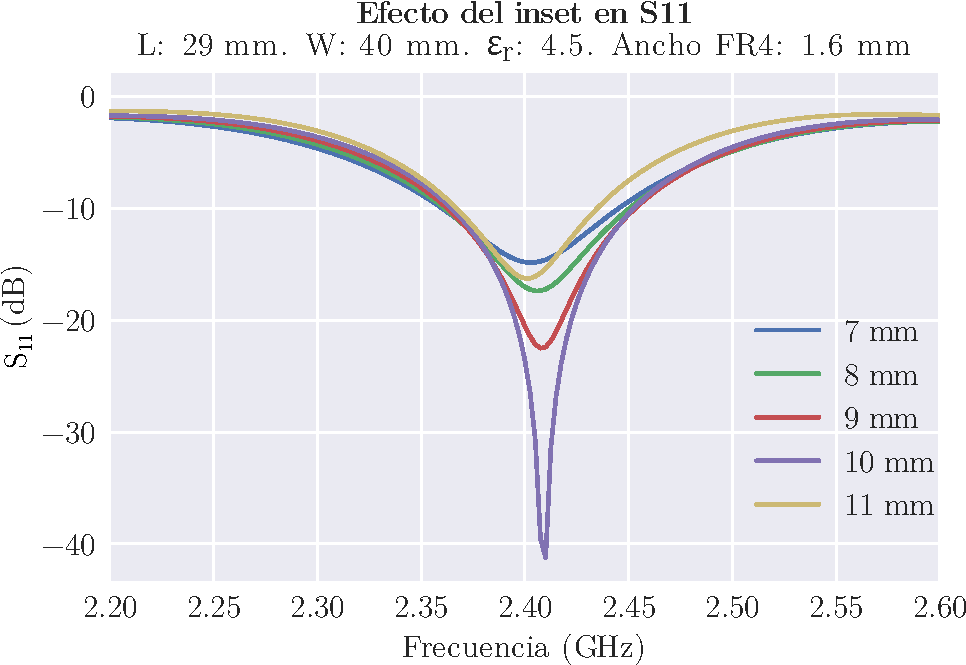
\includegraphics[width=0.48\textwidth]{Aplicacion/VariacionInset-UnParche.pdf}}
	\hspace{19pt}
	\subfigure[Antena sin cargas optimizada.]{
		\label{fig:antena-optimizada}
		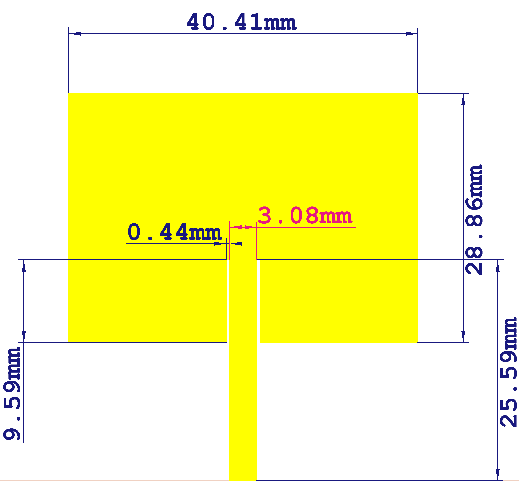
\includegraphics[width=0.42\textwidth]{Aplicacion/antena-optimizada.PNG}}
	\caption{Variación del parámetro $S_{11}$ del puerto en función de distintos parámetros del parche único, y antena optimizada final.}
	\label{fig:simulaciones-microstrip-1parche}
\end{figure}

La variación del valor del ancho W produce efectos menos notorios, modificando ligeramente la frecuencia de resonancia debido a que tiene impacto sobre la longitud efectiva del parche. Además, como se explicó previamente, el ancho del parche modifica la resistencia de entrada, lo que modifica  los valores de $S_{11}$, haciendo que para valores cercanos a 40 mm se obtenga el valor óptimo.

Finalmente, el parámetro de más fácil modificación manual en un parche, el valor del \textit{inset}, da lugar a variaciones muy grandes en el valor del parámetro $S_{11}$. Esto permite una fácil adaptación manual de la antena. Se observa que el valor de \textit{inset} de aproximadamente 10 mm genera los resultados deseados.

La optimización de los parámetros geométricos, realizada con CST Microwave Studio, con objetivo en establecer los valores más adecuados automáticamente para lograr el mínimo valor de $S_{11}$ en 2.41 GHz, arrojó como resultado un valor de L de 28.86 mm, un valor de W de 40.41 mm y un valor de \textit{inset} de 9.59 mm, como se indica en la figura \ref{fig:antena-optimizada}.

En miras de comparar el efecto sobre el campo lejano de las modificaciones a realizarse sobre el parche para aumentar el ancho de banda, se muestra, en la figura \ref{fig:farfield-1parche-sincarga-sinebg}, el comportamiento en campo lejano, donde se asume un sustrato de 190 mm $\times$ 135 mm.

\begin{figure}[h]
	\centering
	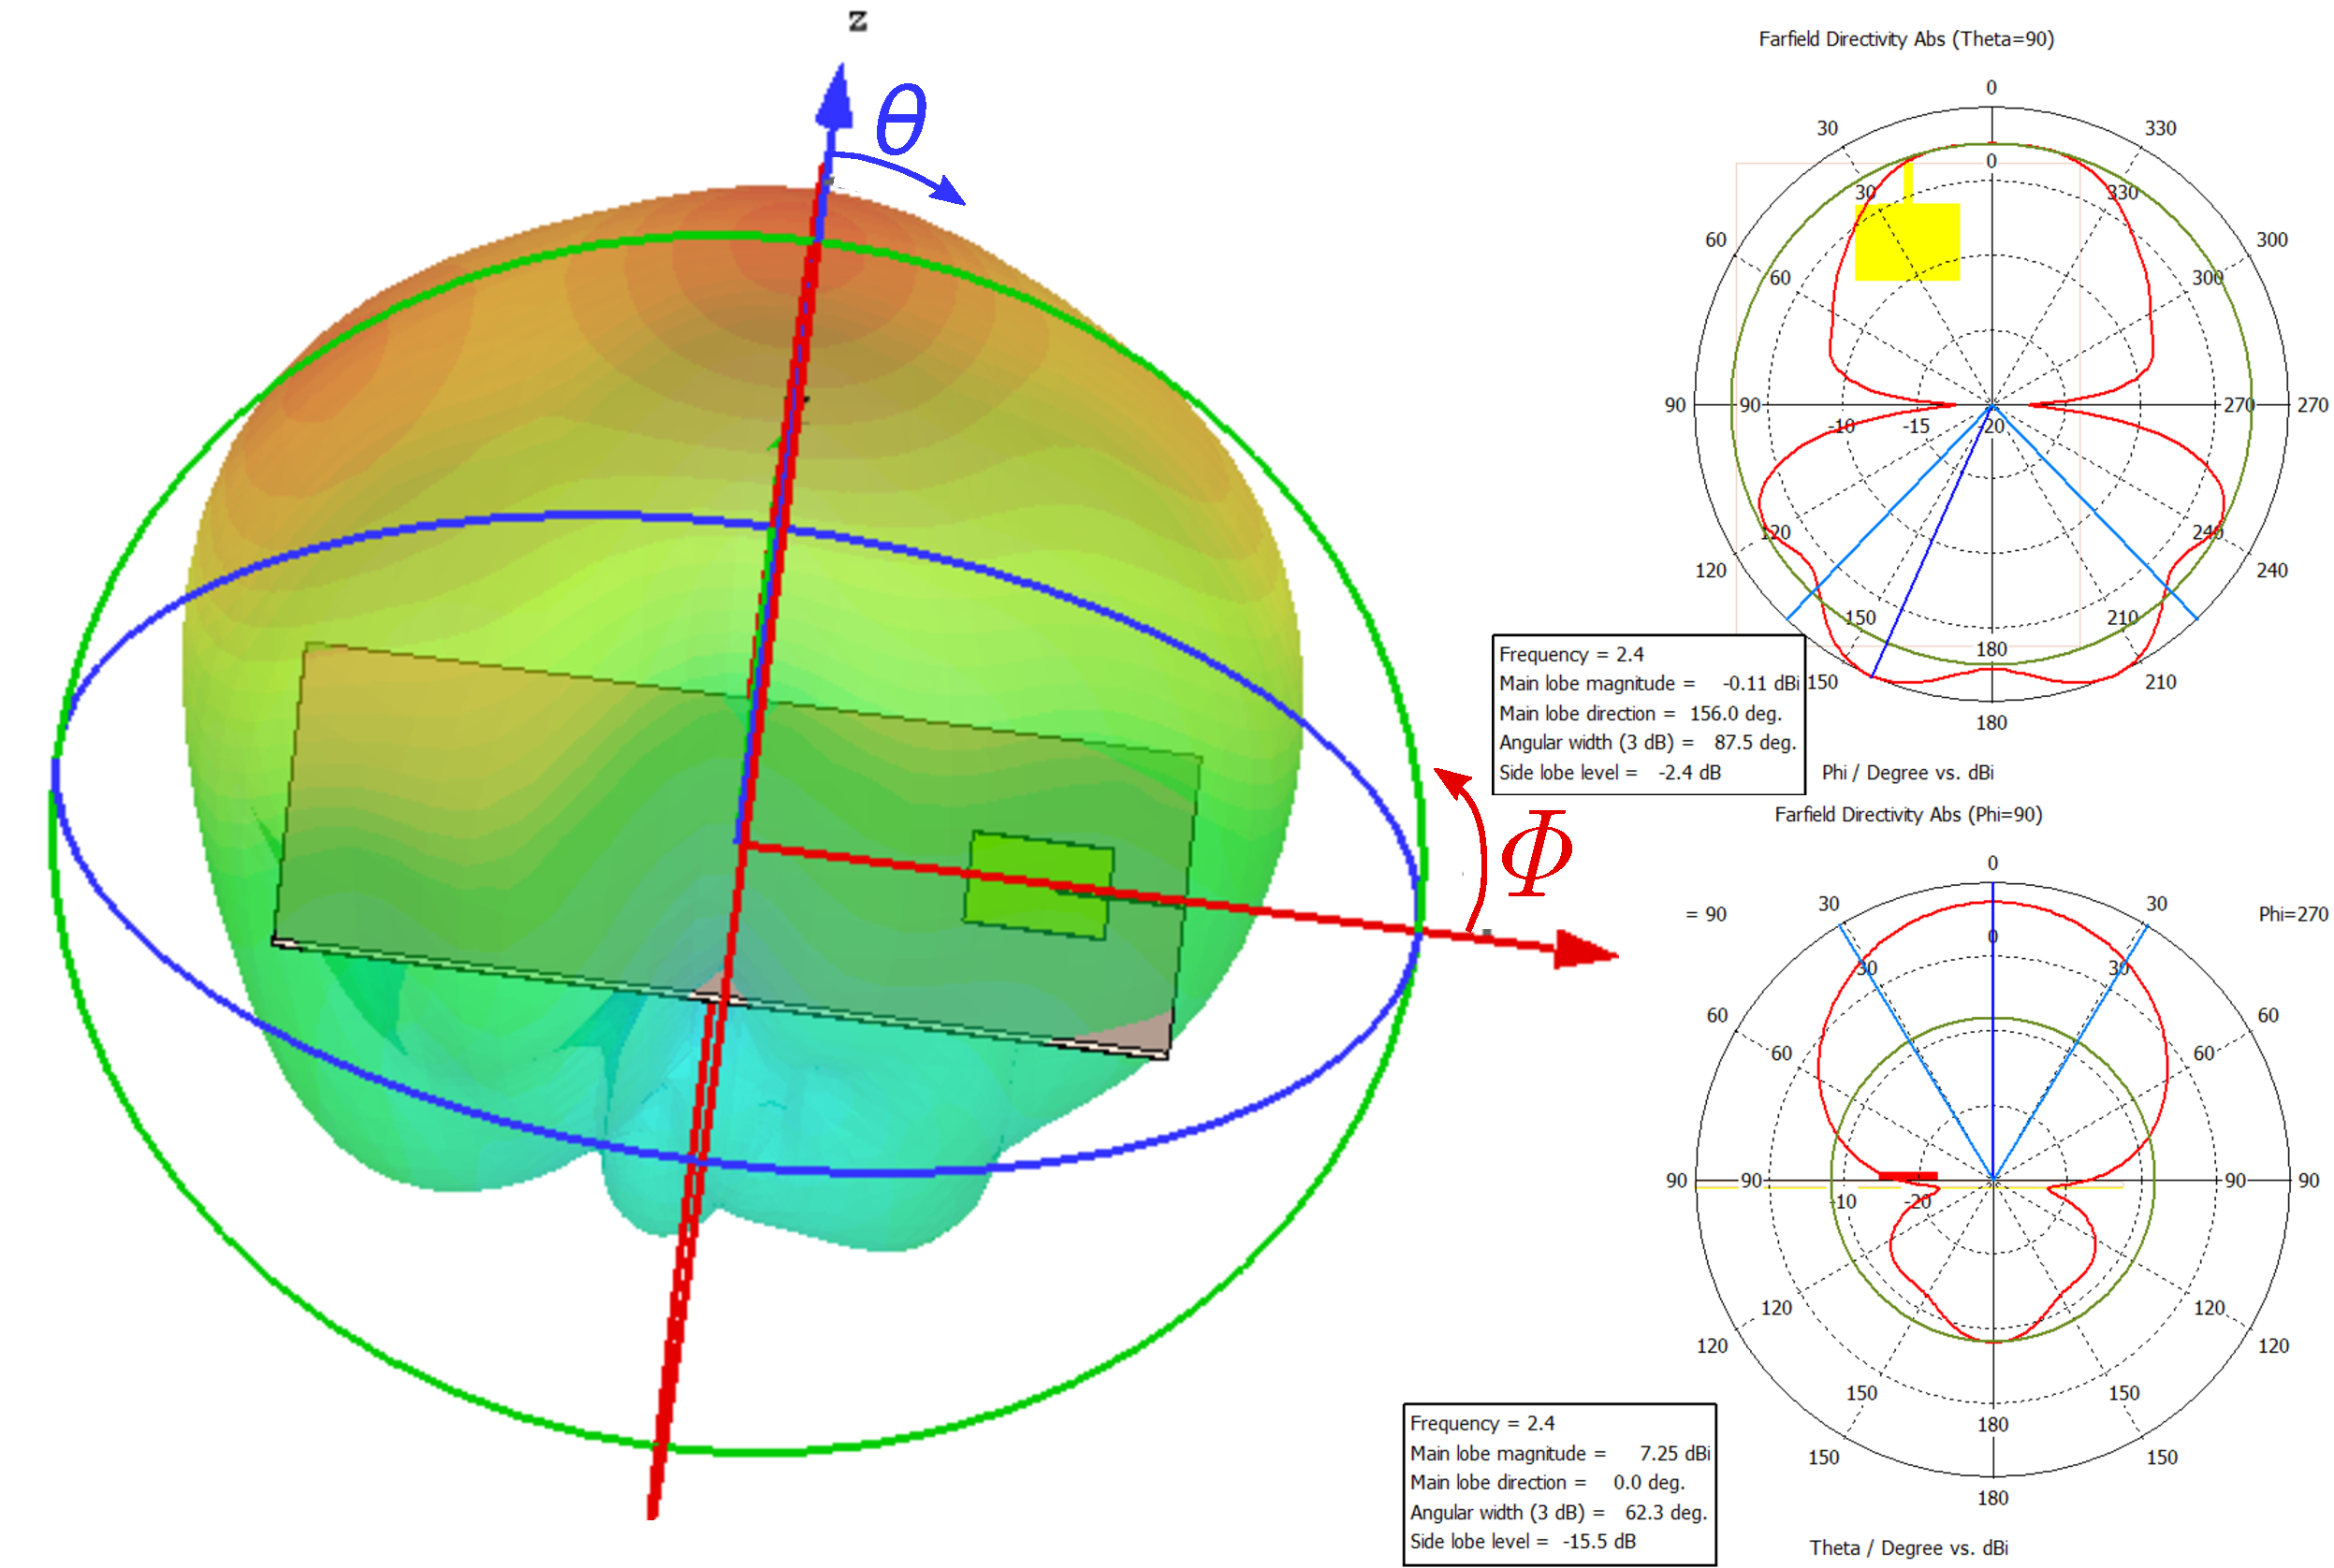
\includegraphics[width=1\textwidth]{Aplicacion/FarfieldResults.pdf}
	\caption{Comportamiento del campo lejano para un parche \textit{microstrip} sin modificaciones, en la frecuencia de resonancia. La imagen tridimensional izquierda muestra la estructura y, en colores, el valor de la directividad para cada dirección. Además, muestra la dirección de variación de $\theta$ y $\phi$. La gráfica superior derecha representa, en rojo, la variación de la directividad en función de $\phi$, para un $\theta$ de $90^{\circ}$, es decir, rasante al plano de la antena. La gráfica inferior derecha representa la variación de la directividad en función de $\theta$, para un valor de $\phi$ de $90^{\circ}$.}
	\label{fig:farfield-1parche-sincarga-sinebg}
\end{figure}


Para poder estudiar este problema, será necesario comprender cómo se comporta un conjunto de dos antenas \textit{microstrip} sin estructuras entre ellas, separadas una distancia adecuada para que los efectos de acoplamiento mutuo resulten visibles. Para evitar, tanto como sea posible, el acoplamiento debido a fenómenos no relacionados a la propagación de ondas de superficie, se debe ubicar a los elementos radiantes a una distancia tal que el diagrama de radiación tenga un comportamiento \textit{broadside}, es decir, que el lóbulo principal del diagrama de radiación tenga dirección perpendicular al plano de tierra. Para esto, la distancia entre las antenas debe ser múltiplo impar de $\lambda_g/2$, donde $\lambda_g$ es la longitud de onda en el sustrato (FR-4, en nuestro caso), donde se considera un valor de $\epsilon_{eff}$ de 4.17. Este valor de permitividad modifica la velocidad de las ondas electromagnéticas, de modo que la longitud de onda, para la frecuencia de resonancia $f_r$ de la antena \textit{microstrip}, es menor a la del vacío. En nuestro caso:

\begin{align}
	\label{eq:lambdag}
	\lambda_g = \frac{v_p}{f_r} = \frac{c}{\sqrt{\epsilon_{eff} f_r}} \approx 60.9\; mm
\end{align}

Considerando que se debe dejar espacio entre las antenas para que se pueda ubicar una estructura EBG entre ellas, se decidió que la distancia entre las mismas resulte de $\frac{3}{2} \lambda_g = 91.35\;mm$.

% Simulaciones en el trabajo.

%% COMO ES ESA DISTANCIA??

% Simular, incluyendo farfield.

% PONER FOTO
% Poner resultados finales

% Condiciones de borde: LIbroSinNombre, pagina 398.
%%%%

\section{Diseño de un conjunto de dos antenas \textit{microstrip}}
\label{sec_conjunto}
El diseño de una única antena microstrip representa el primer paso en la obtención de un conjunto capaz de aumentar la directividad, y por tanto la ganancia, de la estructura. Lamentablemente, la simple utilización de los valores calculados en la sección \ref{sec_disenio_microstrip} no ofrece, en general, buenos resultados. Esto se debe a que las antenas que conforman el conjunto se deben disponer a distancias tales que modifican el espacio circundante a cada una de ellas, generando acoplamiento indeseados y variaciones en la frecuencia de resonancia y los parámetros de adaptación. Es por esto que la sección precedente sólo ofrece valores aproximados a los que se utilizan en el diseño final.

En miras de la obtención de resultados simulados que contemplen las posibilidades de fabricación de un conjunto de dos antenas \textit{microstrip} separadas una distancia de $3/2 \lambda$, se simularon las mismas considerando un sustrato de 135 mm $\times$ 190 mm, de forma que las mismas se ubican a corta distancia del borde de la placa de sustrato utilizada, como se muestra en la figura \ref{fig:conjunto-sin-ebg}. En la misma, los valores de alto, ancho y valor de \textit{inset} de las antenas son iguales, y fueron elegidos tras la simulación a valores cercanos a los obtenidos en la sección anterior. Estos valores, mostrados en la tabla \ref{table:valores-dosparches-geometria}, serán los utilizados para la comparación con las geometrias radiantes con estructuras de banda prohibida electromagnética. En la figura \ref{fig:farfield-2parches-sinebg} se puede observar el diagrama de radiación tridimensional para la estructura propuesta, con las dimensiones elegidas.

\begin{table}
	\centering
	\begin{tabular}{c|c|c|c|c}
		$L$ & $W$ & $y_0$ & $w_{linea}$ & $s$ \\
		\hline
		$31$ mm & $38$ mm & $11$ mm & $3$ mm & $91.35$ mm
	\end{tabular}
	\caption{Tabla de valores elegidos para los parches que conforman al arreglo de dos antenas \textit{microstrip}.}
	\label{table:valores-dosparches-geometria}
\end{table}

GeometriaconjuntoSinEBG.png

FarField3D-DosParches-SinEBG
FarField2D-phifijo-DosParches-SinEBG



\section{Elección del metamaterial}
\label{sec_eleccion}

Existen numerosas posibles celdas unitarias uniplanares, que fueron creadas a partir de la propuesta inicial de Yang y otros \cite{Yang:UCPBG}, y que procuran aumentar el ancho de banda prohibida y el valor de atenuación, muchas veces utilizando técnicas de miniaturización, que buscan lograr geometrías que presenten una mayor o menor inductancia, y una mayor o menor capacidad con el plano de tierra y con celdas vecinas, en función de las necesidades. La búsqueda, en el contexto de la disminución del acoplamiento mutuo entre antenas \textit{microstrip}, de celdas unitarias óptimas, gira alrededor de la búsqueda de anchos de banda prohibidos lo suficientemente amplios para cubrir el ancho de banda de las antenas \textit{microstrip} en cuestión.

Para este trabajo se seleccionó la celda de Yang, analizada en la sección \ref{sec:celda-yang}, debido a que fue la primer variante publicada, y posee optimizaciones sobre la celda de Orlandi, analizada en la sección \ref{sec:celdas-orlandi}.

Sin embargo, existen numerosos diseños y geometrías, entre las que destacan la celda analizada por Goussetis \cite{Goussetis:TailoringAMCEBGCharacteristics}, que consiste en parches cuadrados sin interconexión entre sí, como el mostrado en la figura \ref{fig:rectangulo-cuadrado}. Si bien, debido a su geometría, estas celdas unitarias presentan capacidad con el plano de tierra y con otros parches aledaños, presentan una baja inductancia, lo que los vuelve subóptimos, dado que resulta complejo obtener frecuencias de resonancia lo suficientemente bajas con un tamaño de celda viable. Otros trabajos de interés son los de Abidin \cite{Abidin:Thesis}, quien propuso las estructuras mostradas en las figuras \ref{fig:abidin1} y \ref{fig:abidin2}, que poseen un ancho de banda mayor al de las celdas de Yang, aunque requieren más iteraciones de simulación, debido a la complejidad de las geometrías.

Estructuras más sencillas son propuestas en \cite{Asimonis:designoptimization}, mostradas en las figuras \ref{fig:assimonis1}, \ref{fig:assimonis2} y \ref{fig:assimonis3}, con resultados similares a la geometría elegida en este trabajo.

Entre los esfuerzos más intuitivos para aumentar la inductancia, disminuyendo así la frecuencia de resonancia y, por tanto, el tamaño de las celdas unitarias, se destaca el propuesto por \cite{IslamAlam:CompactEBG}, mostrado en la figura \ref{fig:islamalam}. En ella se observa que se aumentó el largo y la capacidad de las cintas \textit{microstrip} que unen los parches, modificando las líneas para que ocuparan la mayor cantidad de espacio posible. Las simulaciones de esta estructura ofrecen mejores resultados que los de la celda elegida, aunque al costo de dificultar su diseño en programas \textsc{CAD}. Un modelo utilizando líneas de transmisión para caracterizar el comportamiento de estas celdas está presentado en \cite{Venkateswaran:Thesis}. 

En este sentido, \cite{Kovacs:DesignOptimization} propone, en su tesis doctoral, un algoritmo genético capaz de obtener un mayor ancho de banda prohibida mediante sucesivas simulaciones, sin la intervención de un diseñador, obteniendo celdas complejas pero muy efectivas, como la mostrada en la figura \ref{fig:kovacs}.


\begin{figure}[h]
	\centering 
	\subfigure[Celda unitaria propuesta por \cite{Abidin:Thesis}.]{
		\label{fig:abidin1}
		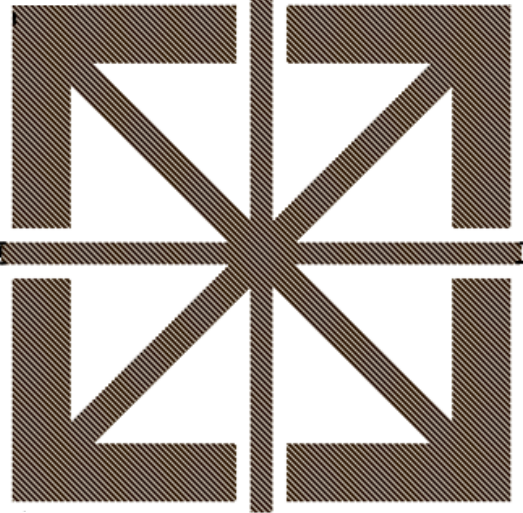
\includegraphics[width=0.30\textwidth]{Aplicacion/abidin1.png}}
	\hspace{30pt}
	\subfigure[Celda unitaria propuesta por \cite{Abidin:Thesis}.]{
		\label{fig:abidin2}
		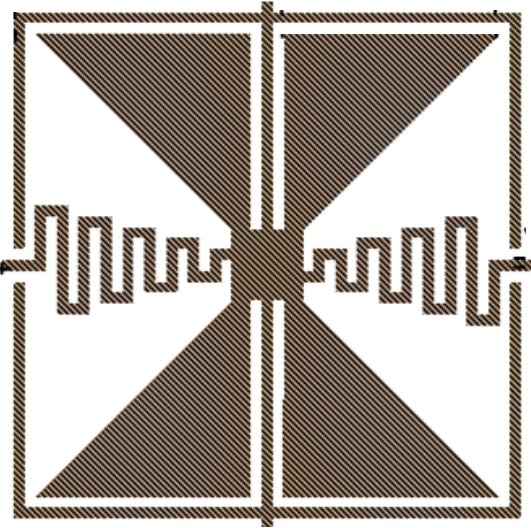
\includegraphics[width=0.30\textwidth]{Aplicacion/abidin2.png}}
	\subfigure[Celda unitaria propuesta por \cite{Asimonis:designoptimization}.]{
		\label{fig:assimonis1}
		
\includegraphics[width=0.30\textwidth]{Aplicacion/assimonis1.png}}
	\hspace{30pt}
	\subfigure[Celda unitaria propuesta por \cite{Asimonis:designoptimization}.]{
		\label{fig:assimonis2}
		
\includegraphics[width=0.30\textwidth]{Aplicacion/assimonis2.png}}
	\subfigure[Celda unitaria propuesta por \cite{Asimonis:designoptimization}.]{
		\label{fig:assimonis3}
		
\includegraphics[width=0.30\textwidth]{Aplicacion/assimonis3.png}}
	\hspace{30pt}
	\subfigure[Celda unitaria propuesta por \cite{IslamAlam:CompactEBG}.]{
		\label{fig:islamalam}
		
\includegraphics[width=0.30\textwidth]{Aplicacion/islamalam.png}}
	\subfigure[Celda unitaria propuesta por \cite{Kovacs:DesignOptimization}.]{
		\label{fig:kovacs}
		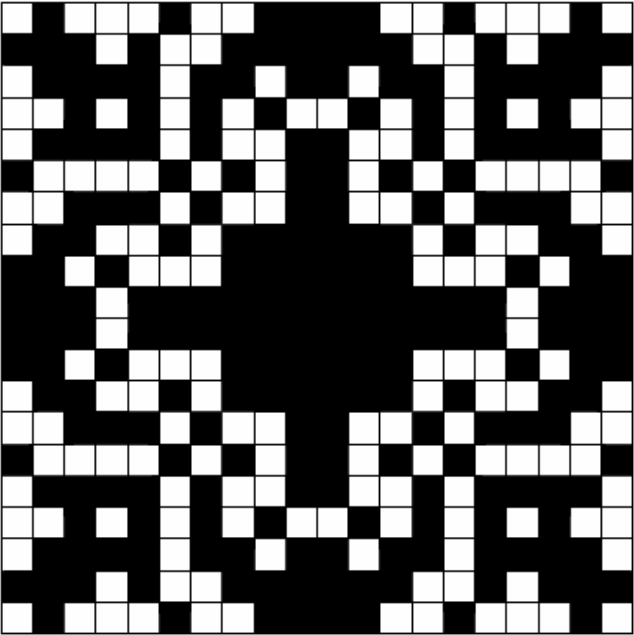
\includegraphics[width=0.30\textwidth]{Aplicacion/kovacs.png}}
	\caption{Variación del parámetro $S_{11}$ del puerto en función de distintos parámetros del parche único, y antena optimizada final.}
	\label{fig:simulaciones-microstrip-1parche}
\end{figure}

La miniaturización cumple un papel importante debido a que es necesaria una cantidad (o profundidad) mínima de celdas unitarias entre los parches para que el efecto de disminución de acoplamiento resulte notorio. Si cada una de las celdas unitarias ocupara demasiada superficie, obligaría a separar los parches aún más, consecuencia que resulta indeseable. Además, entre la estructura de celdas unitarias y los parches se debe mantener una distancia $g$ mínima, de modo que los efectos de acoplamiento de campo cercano entre la antena y la estructura EBG puedan considerarse despreciables. Estos efectos no son despreciables y, en muchos casos, generan un acoplamiento aún mayor al que se da si no se utilizan estructuras EBG.

Para el caso de una distancia entre los parches de aproximadamente $3\lambda/2$, la cantidad de filas de celdas unitarias que se pueden ubicar entre los mismos para observar efectos de atenuación del acoplamiento mutuo varía entre 3 y 5. Las técnicas de modelado presentadas, y en particular las que requieren de simulación de una celda unitaria y la aplicación de condiciones de borde periódicas, describen el comportamiento de la estructura EBG cuando ésta se extiende infinitamente. Como, en general, este no es el caso, se procedió, utilizando como base la información brindada por los diagramas de dispersión (que en nuestro caso, debido a que la cantidad de celdas unitarias es finita, describen en forma aproximada las zonas frecuencia de atenuación), a obtener la relación del parámetro $S_{21}$ con la frecuencia para distintos valores geométricos, simulando la estructura completa.

De los parámetros analizados que describen la geometría de las celdas unitarias de Yang, para ambos análisis (el que corresponde a la resolución de una única celda unitaria con condiciones de contorno periódicas, y el que simula una estructura finita completa), los más importantes resultaron: el tamaño de la celda unitaria, el tamaño del parche central y la distancia entre los parches de dos celdas unitarias aledañas.

En general, un mayor tamaño de celda da lugar a una banda de atenuación ubicada a frecuencias más bajas. La elección gira en torno a que la frecuencia de resonancia del sistema sobre el que se desea probar el comportamiento de la estructura se ubique en una zona segura ante problemas y tolerancias de fabricación.

\section{Estudio del efecto de la distancia sobre el ancho de banda}
\label{sec_efecto_distancia}
%%%%
%Coccioli, Yang, Itoh, pag 2127 -> básicamente dice que afecta, que disminuye la frecuencia de resonancia del parche si están demasiado cerca.
% Iluz, Shavit, pag 1448

Finalmente, es necesario agregar las estructuras EBG para observar el efecto que producen en el arreglo de antenas. Para ello, en primer lugar se debe reducir el efecto que las estructuras ejercen sobre cada uno de los parches por separado, para lo cual también se realizó un conjunto de simulaciones, donde las estructuras se ubicaron a distintas distancias de la antena ($g$ en la figura \ref{fig:antena-propuesta-con-ebg}).

% Creo que va a pasar esto
Como se puede observar, una mayor cercanía entre la estructura EBG y la antena radiante disminuye la frecuencia de resonancia de la misma, debido a los efectos de acoplamiento mutuo.
% PUede ir esto
% De las gráficas de la figura, se puede concluir que, si se buscan disminuir el acoplamiento mutuo entre antenas que están cerca mediante la reducción de ondas de superficie, resulta importante considerar, en el diseño de las antenas, a la estructura EBG utilizada, debido que la misma modifica parámetros importantes de la antena.
% O puede ir esto
% De las gráficas de la figura, se puede concluir que, si se buscan disminuir el acoplamiento mutuo entre antenas que están cerca mediante la reducción de ondas de superficie, se debe ubicar a la estructura EBG a una distancia tal que los efectos de acoplamiento mutuo sean despreciables para cada antena y para el diagrama de radiación.

\section{Estudio del efecto sobre el acoplamiento mutuo}
\label{sec_estudio_acoplam_mutuo}
%%%%
Establecida la distancia adecuada, es posible ahora incorporar a la simulación las estructuras EBG para observar el efecto sobre el acoplamiento mutuo. Se debe tener en cuenta que la cantidad de celdas unitarias debe ser suficiente para lograr el efecto de reducción del acoplamiento mutuo.


% Ondas de superficie se proparagan por plano E? Pagina 132. Rahmat, lbro,.
% Pagina 138. Rahmat.
% Efecto según la orientacion de parches. ABidin, Tesis, Pagina 37.
% Algo se puede ver en Assimonis, Yioultsis, Antonopoulos
%%%%


% Ver que overall las conclusiones son similares a Islam,Alam.
